%% Aide-mémoire
\documentclass[french, landscape]{article}
%% -----------------------------
%% Préambule
%% -----------------------------
%% Bug avec les accents dans la définition des variables ici, à voir plus tard.

% !TEX encoding = UTF-8 Unicode
% LaTeX Preamble
% Author : Gabriel Crépeault-Cauchon

% HOW-TO : copy-paste this file in the same directory as your .tex file, and add in your preamble the next command right after you have specified your documentclass : 
% \input{preamble-cheatsht.tex}
% ---------------------------------------------
% ---------------------------------------------

%% -----------------------------
%% Encoding packages
%% -----------------------------
\usepackage[utf8]{inputenc}
\usepackage[T1]{fontenc}
\usepackage{babel}
\usepackage{lmodern}

%% -----------------------------
%% Variable definition
%% -----------------------------


\def\session{Automne 2018}
\def\auteur{Gabriel Crépeault-Cauchon // Nicholas Langevin}
\def\BackgroundColor{white}


%% -----------------------------
%% Margin and layout
%% -----------------------------
% Determine the margin for cheatsheet
\usepackage[landscape, hmargin=1cm, vmargin=1.7cm]{geometry}
\usepackage{multicol}

% Remove automatic indentation after section/subsection title.
\setlength{\parindent}{0cm}

% Save space in cheatsheet by removing space between align environment and normal text.
\usepackage{etoolbox}
\newcommand{\zerodisplayskips}{%
  \setlength{\abovedisplayskip}{0pt}%
  \setlength{\belowdisplayskip}{0pt}%
  \setlength{\abovedisplayshortskip}{0pt}%
  \setlength{\belowdisplayshortskip}{0pt}}
\appto{\normalsize}{\zerodisplayskips}
\appto{\small}{\zerodisplayskips}
\appto{\footnotesize}{\zerodisplayskips}

%% -----------------------------
%% URL and links
%% -----------------------------
\usepackage{hyperref}
\hypersetup{colorlinks = true, urlcolor = gray!70!white, linkcolor = black}

%% -----------------------------
%% Document policy (uncomment only one)
%% -----------------------------
%	\usepackage{concrete}
	\usepackage{mathpazo}
%	\usepackage{frcursive} %% permet d'écrire en lettres attachées
%	\usepackage{aeguill}
%	\usepackage{mathptmx}
%	\usepackage{fourier} 

%% -----------------------------
%% Math configuration
%% -----------------------------
\usepackage[fleqn]{amsmath}
\usepackage{amsthm,amssymb,latexsym,amsfonts}
\usepackage{empheq}
\usepackage{numprint}

% Mathematics shortcut
\newcommand{\reels}{\mathbb{R}}
\newcommand{\entiers}{\mathbb{Z}}
\newcommand{\naturels}{\mathbb{N}}
\newcommand{\eval}{\biggr \rvert}
\usepackage{cancel}
\newcommand{\derivee}[1]{\frac{\partial}{\partial #1}}
\newcommand{\prob}[1]{\Pr \left( #1 \right)}
\newcommand{\esp}[1]{\mathrm{E} \left[ #1 \right]}
\newcommand{\variance}[1]{\mathrm{Var} \left( #1 \right)}
\newcommand{\covar}[1]{\mathrm{Cov} \left( #1 \right)}
\newcommand{\laplace}{\mathcal{L}}

% To indicate equation number on a specific line in align environment
\newcommand\numberthis{\addtocounter{equation}{1}\tag{\theequation}}

% Actuarial notation package
\usepackage{actuarialsymbol}
\usepackage{actuarialangle}

% Matricial anotation for math symbols (\bm{•})
\usepackage{bm}
% matricial notation variable (bold style)
\newcommand{\matr}[1]{\mathbf{#1}}



%% -----------------------------
%% tcolorbox configuration
%% -----------------------------
\usepackage{tcolorbox}
\tcbuselibrary{xparse}
\tcbuselibrary{breakable}

%% Définition boite pour définition
\DeclareTColorBox{definition}{ o }% #1 parameter
{colframe=blue!60!green,colback=blue!5!white, % color of the box
breakable, pad at break*=0mm, % to split the box
title = {#1},
after title = {\large \hfill \faBook}
}

%% -----------------------------
%% Graphics and pictures
%% -----------------------------
\usepackage{graphicx}
\usepackage{pict2e}

%% -----------------------------
%% insert pdf pages into document
%% -----------------------------
\usepackage{pdfpages}

%% -----------------------------
%% Color configuration
%% -----------------------------
\usepackage{color, soulutf8, colortbl}


% New color definition
% Source : http://latexcolor.com


% usefull shortcut for colored text
\newcommand{\orange}{\textcolor{orange}}
\newcommand{\red}{\textcolor{red}}
\newcommand{\cyan}{\textcolor{cyan}}
\newcommand{\blue}{\textcolor{blue}}
\newcommand{\green}{\textcolor{green}}
\newcommand{\purple}{\textcolor{magenta}}
\newcommand{\yellow}{\textcolor{yellow}}


%% -----------------------------
%% Enumerate environment configuration
%% -----------------------------
% Custum enumerate & itemize Package
\usepackage{enumitem}
% French Setup for itemize function
\frenchbsetup{StandardItemLabels=true}
% Change default label for itemize
\renewcommand{\labelitemi}{\faAngleRight}

%% -----------------------------
%% Tabular column type configuration
%% -----------------------------
\newcolumntype{C}{>{$}c<{$}} % math-mode version of "l" column type
\newcolumntype{L}{>{$}l<{$}} % math-mode version of "l" column type
\newcolumntype{R}{>{$}r<{$}} % math-mode version of "l" column type
\newcolumntype{f}{>{\columncolor{green!20!white}}p{1cm}}
% configuration to force a line break within a single cell
\usepackage{makecell}



%% -----------------------------
%% Fontawesome for special symbols
%% -----------------------------
\usepackage{fontawesome}

%% -----------------------------
%% Section Font customization
%% -----------------------------
\usepackage{sectsty}
\sectionfont{\color{\SectionColor}}
\subsectionfont{\color{\SubSectionColor}}

%% -----------------------------
%% Footer/Header Customization
%% -----------------------------
\usepackage{lastpage}
\usepackage{fancyhdr}
\pagestyle{fancy}
% Header
\fancyhead{} 	% Reset
\fancyhead[L]{Aide-mémoire pour~ \cours ~(\textbf{\sigle})}
\fancyhead[R]{\auteur}

% Footer
\fancyfoot{}		% Reset
\fancyfoot[R]{\thepage ~de~ \pageref{LastPage}}
\fancyfoot[L]{\href{https://github.com/gabrielcrepeault/latex-template}{\faGithub \ gabrielcrepeault/latex-template}}

% page background color
\pagecolor{\BackgroundColor}






%% END OF PREAMBLE
% ---------------------------------------------
% ---------------------------------------------


% Couleur de la page
%\pagecolor{gray!10!white}
\newcolumntype{a}{>{\columncolor{red!20!white}$}p{2cm}<{$}}

%% -----------------------------
%% Début du document
%% -----------------------------
\begin{document}

\small
\begin{multicols*}{3} % Nombre de colonnes (peut être changé plus tard.)

\setcounter{section}{2}
\section{Estimation non-paramétrique}
\subsection*{Moments à savoir}
\begin{align*}
\mu_k^{\prime} 	& = \esp{X^k} \\
\mu_k			& = \esp{(X-\mu)^k} \\
CV				& = \frac{\sigma}{\mu} \\
\gamma			& = \frac{\mu_3}{\sigma^3}  \\
\kappa			& = \frac{\mu_4}{\sigma^4} \\
\end{align*}

\subsection*{3 critères pour évaluer les queues de distributions}

\begin{enumerate}

\item La loi avec le moins de moments a la queue la plus lourde.
\item Première à diverger du quotient des distributions a la queue la plus lourde.
\[\lim_{x \to \infty} \frac{f_{X_1}(x)}{f_{X_2}(x)}\]
\item Si la fonction hasard $h(x) = \frac{f_X(x)}{S_X(x)}$ est croissante alors la queue est fine, sinon elle est lourde.
\[
\begin{matrix}
	h_X'(x) < 0 & \text{queue lourde} \\
	h_X'(x) > 0 & \text{queue fine} \\
\end{matrix}
\]
\end{enumerate}


\subsection*{Quantités des distributions à connaître}

\begin{itemize}
\item[$Y^P$ : ] 
	\textbf{Excess loss}, alias \textbf{left truncated} and \textbf{shifted} variable. \\
	On interprete comme le \textit{montant de perte} en \textit{excès d'un déductible d} sachant que la perte est au delà de ce montant.


\item[$Y^L$ : ] 
	\textbf{Left censored} and \textbf{shifted} variable. \\ 
	Elle est défini comme étant 0 pour toutes les pertes inférieures à d, alors que l'excès-moyen n'est simplement pas défini dans ces cas. \\
	Donc, celle-ci a une masse à 0.


\item[$Y$ : ] 
	\textbf{Limited loss}, alias \textbf{right censored} variable. \\ 
	


	\begin{itemize}
		\item[\textbf{shifted} :] d est soustrait des valeurs restantes. \\
		On peut visualiser le déplacement de la courbe de densité à la gauche.
		\item[\textbf{left truncated} :] Toutes valeurs inférieures à d ne sont pas observées.			\item[\textbf{left censored} :] Toutes valeurs inférieures à d sont égale à 0.
		\item[\textbf{right censored} :] Toutes valeurs supérieures à u sont égale à u.
	\end{itemize}	
\end{itemize}


\begin{itemize}
\item[] \textbf{Moments}
\begin{align*}
	\esp{Y^P} &= \esp{X-d | X \geq d} = \frac{\int_{d}^{\infty} S_X(x)}{S_X(d)} = e_X(d) \\
	\esp{Y^L} &= \esp{(X - d)_+} = \int_{d}^{\infty} (x - d) f_X(x) dx \\
	\esp{Y} &= E[X \wedge d] = \int_0^d f_X(x) dx \Leftrightarrow \int_0^d S_X(x) dx
\end{align*}

%\item[] \textbf{Définitions des variables}
%\begin{align*}
%Y^P 	&= ( X - d | X > d ) 
%	&= 
%	\left\{
%		\begin{array}{ll}
%			\text{undefined}, 	& X \leq d \\
%			X - d, 				& X > d
%		\end{array}
%	\right. \\
%Y^L 	&= ( X - d )_+ 
%	&= 
%	\left\{
%		\begin{array}{ll}
%			0, 		& X \leq d \\
%			X - d, 	& X > d
%		\end{array}
%	\right. \\
%Y 	&= (X \wedge u)
%	&= 
%	\left\{
%		\begin{array}{ll}
%			X, & X < u \\
%			u, & X \geq u
%		\end{array}
%	\right.
%\end{align*}
\end{itemize}

\setcounter{section}{7}
\section{Fréquence et sévérité avec modifications aux contrats}
\subsection*{Déductible ordinaire}

\subsubsection*{L'assureur paye tout montant en excédent du montant d.}
%\setlength{\abovedisplayskip}{-20pt}
%\setlength{\belowdisplayskip}{20pt}
\begin{align*}
Y^L &= (X-d)_+ = 
	\begin{cases}
		0		& , X \leq d \\
		X - d	& , X > d \\
	\end{cases} \\
Y^P &= (X-d)_+ = 
	\begin{cases}
		\text{Non-défini}	& , X \leq d \\
		X - d				& , X > d \\
	\end{cases}
\end{align*}

\subsection*{Déductible franchise}
\subsubsection*{L'assureur paye l'entièreté des coûts pour toute perte qui surpasse le montant d.\\ \textit{Pour éviter les petites réclamations}}
\begin{align*}
Y^L &= (X-d)_+ = 
	\begin{cases}
		0		& , X \leq d \\
		X		& , X > d \\
	\end{cases} \\
Y^P &= (X-d)_+ = 
	\begin{cases}
		\text{Non-défini}	& , X \leq d \\
		X 					& , X > d \\
	\end{cases}
\end{align*}

\subsubsection*{Moments}
\begin{align*}
E[Y_{(O\textcolor{red}{|F)}}^{(L\textcolor{blue}{|P)}}] &= \frac{E[X] - E[X \wedge d] + \textcolor{red}{d S_X(d)} }{\textcolor{blue}{S_X(d)}} \\
\end{align*}
Où (L|P) et (O|F) est à être interprété en REGEX. \\
C'est soit per loss (L) ou \textcolor{blue}{per payment (P)} \\
C'est soit un déductible ordinaire (O) ou \textcolor{red}{avec franchise (F)}.
De plus, on note que:
\begin{align*}
E[Y_{(O)}^{(\textcolor{blue}{P)}}] &= e_X(d) \\
E[Y_{(O)}^{(L)}] &= \pi_X(d)
\end{align*}

\subsubsection*{Fonctions}
\begin{align*}
f_{Y^{(L\textcolor{blue}{|P)}}_{(O)}} &= \frac{f_X(y+d)}{\textcolor{blue}{S_X(d)}} \\
S_{Y^{(L\textcolor{blue}{|P)}}_{(O)}} &= \frac{S_X(y+d)}{\textcolor{blue}{S_X(d)}} \\
F_{Y^{(L\textcolor{blue}{|P)}}_{(O)}} &= \frac{F_X(y+d) \textcolor{blue}{- F_X(d)}}{\textcolor{blue}{S_X(d)}} \\
h_{Y^{(Y|P)}_{(O)}} &= h_X(y+d) \\
\end{align*}


\subsection*{LER et inflation du déductible ordinaire}
%\subsubsection*{}
Le LER nous donne le pourcentage de perte qu'on ne paie pas grâce au déductible
\begin{align*}
	LER 	 &= \frac{\esp{X} - \esp{(X-u)_+}}{\esp{X}} \\
	     &= \frac{\esp{X \wedge u}}{\esp{X}} \\
\end{align*}
Soit $X^I = (1 + r) X$
\begin{align*}
	E[{X^I} \wedge u]	 &= (1 + r) E[X \wedge \frac{u}{1 + r}] \\
	f_{X^I}(x) &= \frac{f_X\left(\frac{y}{1 + r}\right)}{1 + r} \\
	F_{X^I}(x) &= F_X\left(\frac{y}{1 + r}\right)
\end{align*}

\subsection*{Limite de police}
\subsubsection*{L'assureur paye un maximum de $u$}

\begin{align*}
Y 	&= (X \wedge u)
	= 
	\left\{
		\begin{array}{ll}
			X, & X < u \\
			u, & X \geq u
		\end{array}
	\right. \\
f_Y(y) &=
		\left\{
			\begin{array}{ll}
				f_X(y), & y < u \\
				S_X(u), & y = u
			\end{array}
		\right. \\
F_Y(y) &=
		\left\{
			\begin{array}{ll}
				F_X(y), & y \leq u \\
				1, & y > u
			\end{array}
		\right. \\
\end{align*}

\subsection*{Coassurance}
\subsubsection*{L'assureur paye une fraction, $\alpha$, de la perte.}

Si la coassurance est la seule modification, alors nous obtenons $Y = \alpha X$. \\
\textit{L'impact sur les fonctions est le même qu'avec de l'inflation}.

\subsection*{Formule récapitulative}
\subsubsection*{Lorsque les 4 items sont présent (déductible \textit{ordinaire}, limite, inflation et coassurance.}

\begin{align*}
Y^L = 
\begin{cases}
0		& ,\ x  < \frac{d}{1+r} \\
\alpha \Big( (1+r) x - d \Big)	& ,\ \frac{d}{1+r} \leq x < \frac{u}{1+r} \\
\alpha (u-d)		& ,\ x \geq \frac{u}{1+r} \\
\end{cases}
\end{align*}
\begin{align*}
Y^P = 
\begin{cases}
\text{Non-défini}		& ,\ x  < \frac{d}{1+r} \\
\alpha \Big( (1+r) x - d \Big)	& ,\ \frac{d}{1+r} \leq x < \frac{u}{1+r} \\
\alpha (u-d)		& ,\ x \geq \frac{u}{1+r} \\
\end{cases}
\end{align*}

\begin{align*}
\esp{Y^L} &= \alpha (1+r) \left( \esp{X \wedge \frac{u}{1+r}} - \esp{X \wedge \frac{d}{1+r}}   \right) \\
\esp{Y^P} &= \frac{\esp{Y^L}}{S_X \left( \frac{d}{1+r} \right)}
\end{align*}

\setcounter{section}{13}
\section{Estimation non-paramétrique des fonctions de répartition et de survie}
\begin{align*}
F_n(x) &= \frac{1}{n} \sum\limits_{j=1}^n I_{\{ x_j \leq x\}} \\
f_n(x) &= \frac{1}{n} \sum\limits_{j=1}^n I_{\{ x_j = x\}}  \\
 n F_n&(x)  \sim \text{bin}(n, F(x))\\
E[F_n(x)] &= \frac{n F_n(x)}{n} = F_n(x)\\
\widehat{Var}[F_n(x)] &= \frac{n F_n(x)(1 - F)n(x)}{n^2} \\
       &= \frac{F_n(x)(1 - F_n(x))}{n}  \\
\widehat{Var}[S_n(x)] &= \frac{S_n(x)(1 - S_n(x))}{n} \\
F_n(x) &= 
\left\{
	\begin{array}{ll}
		0,  &  x < y_1 \\
        1 - \frac{r_j}{n}, &  y_{j-1} \leq x < y_j, j=2,...,k \\
        1, & x > y_k 
	\end{array}
\right.
\end{align*}

\subsection*{Estimateur de Nelson-Aalen}
% Formules à valider, je ne crois pas avoir pris les bonnes dans le Loss Models
%\begin{itemize}
%    \item L'estimateur de Nelson–Aalen est une alternative à la fonction de répartition empirique comme estimateur de la fonction de survie dans le cas de données complètes.
%\end{itemize}
%\begin{align*}
%    h(x) &= -ln S(x) \\
%    \hat{H}(x) &= 
%    \left\{
%	\begin{array}{ll}
%		0,  &  x < y_1 \\
%        \sum\limits_{i=1}^{j-1} \frac{s_i}{r_i}, &  y_{j-1} \leq x < y_j, j=2,...,k \\
%        \sum\limits_{i=1}^{k} \frac{s_i}{r_i}, & x > y_k 
%	\end{array}
%\right. \\
%\hat{S}(x) &= e^{-\hat{H}(x)} \\
%\frac{s_i}{r_i} &= \frac{s_i/n}{r_i/n} \\
%                &= \frac{s_i/n}{1 - (1 - F_n(y_{i-1}))} \\
%                &= \frac{f_n(y_i)}{1 - (1 - F_n(y_{i-1}))} \\
%E[\hat{H}(y_j)] &= H(y_j) \\
%\widehat{Var}[\hat{H}(y_j)] &\approx \sum_{i=1}^j \frac{s_i}{r_i^2} 
%\end{align*}

\subsection*{Estimateur de Kaplan-Meier}
% à corriger et revoir le layout
%\begin{align*}
%    r_i &= \text{\# sujets sortis du groupe à ou après $y_i$} \\
%        &= \text{\# sujets non encore entrés dans le groupe à $y_i$} \\
%    \hat{S}(x) &=
%    \left\{
%	\begin{array}{ll}
%		1,  &  0 \leq x < y_1 \\
%        \prod\limits_{i=1}^{j-1} \frac{r_i - s_i}{r_i}, &  y_{j-1} \leq x < y_j, j=2,...,k \\
%        \prod\limits_{i=1}^{k} \frac{r_i - s_i}{r_i}, & x > y_k \: \text{(0 si données complètes)}
%	\end{array}
%    \right. \\
%    E[\hat{S}(x)] &= \frac{S(y_i)}{S(y_1)}\: \text{i.e. sans biais à $y_i$} \\
%    \widehat{Var}[\hat{S}(y_j)] &= [\hat{S}(y_j)]^2 \sum_{i=1}^j \frac{s_i}{r_i(r_i - s_i)}\: \textbf{(Aprox. GreenWood)}
%\end{align*}


\section{Fonction génératrice cumulante}
Soit la fonction génératrice des moments $M_X(t)$, telle que
\[M_X(t) = \esp{e^{tX}}\]
Alors, la fonction génératrice cumulante $K_X(t)$ est définie comme
\[K(t) = \derivee{t} \ln M_X(t)\]
De plus, la fonction génératrice cumulante a les propriétés suivantes : 
\begin{align*}
K'(t) \eval_{t = 0} & =   \esp{X} \\
K''(t) \eval_{t=0} & = \variance{X} \\
\end{align*}


\section{Frequentist estimation}
\subsection*{Méthode des moments}
On résoud $p$ équations à $p$ inconnus, telles que
\[\hat{\mu}_k' = \mu_k'\]

\subsection*{Méthode des percentiles}
On résoud $p$ équations à $p$ inconnus (paramètres) telles que
\[F_n(\hat{\pi}_{g_i}) = g_i \quad  i = 1, ..., p\]
où $\hat{\pi}_{g_i}$ est le $g_i$\up{e} quantile de la fonction empirique.

\subsubsection*{Smoothed empirical estimate}
Parfois, le quantile recherché tombe entre 2 \emph{marches} de la fonction empirique. On utilise l'approximation linéaire suivante avec les statistiques d'ordre $X_{(j)}$ : 
\[\hat{\pi}_{g}  = (1-h)X_{(j)} + h X_{(j+1)} \]
avec $j = \lfloor (n+1)g \rfloor$ et $h = (n+1) g - j$.

\subsection*{Méthode du maximum de vraisemblance (\emph{MLE})}
\subsubsection*{Données complètes}
On définit la fonction de vraisemblance  $L(\theta)$telle que
\[L(\theta) = \prod_{i=1}^{n} f(x_i ; \theta)\]
Et la fonction de log-vraisemblance $\ell(\theta)$
\[\ell(\theta) = \sum_{i=1}^{n}  \ln f(x_i ; \theta) \]
L'estimateur du maximum de vraisemblance $\bm{\theta}$ maximiser $L(\theta)$ ou $\ell(\theta)$, i.e.
\[\derivee{\theta} \ell(\theta) \eval_{\theta = \hat{\theta}_{MLE}}  = 0\]

\subsubsection*{Données groupées}
Si les données sont groupées, alors on utilise une forme plus générale de la fonction de vraisemblance : 
\[L(\theta) =  \prod_{j=1}^{k}  \left( F_X(c_{j} ; \theta) - F_X(c_{j-1} ; \theta) \right)^{n_j}   \]
où $F_X$ est la fonction de répartition théorique de la distribution qu'on suppose la distribution de notre estimateur \emph{MLE}. Si les données sont censurés à la classe $c_{j-1}$, alors on utilise $(1-F_X(c_{j-1}; \theta))$.

\subsection*{Variance des estimateurs et intervalle de confiance}



\subsubsection*{Estimation de la variance de $\hat{\theta}$}
L'information de Fisher $I(\theta)$ est définie par
\[I(\theta) = -\esp{\frac{\partial^2}{\partial \theta^2} \ell(\theta)} = \esp{\left( \derivee{\theta} \ell(\theta) \right)^2}\]
Si l'information n'est pas connue, on peut l'estimer avec \emph{l'information observée} : 
\[\hat{I}(\hat{\theta}) = \sum_{i=1}^{n} \left( \derivee{\theta} \ln f(x_i ; \theta) \eval_{\theta = \hat{\theta}} \right)^2 = - \sum_{i=1}^{n}  \frac{\partial^2}{\partial \theta^2} \ln f(x_i ; \theta) \eval_{\theta = \hat{\theta}}\]
Ainsi, on peut calculer la variance de l'estimateur $\hat{\theta}_{MLE}$ telle que
\[\variance{\hat{\theta}} = I(\theta)^{-1}\]

\subsubsection*{Intervalle de confiance pour $\hat{\theta}$}
Lorsque $n \to \infty$, $\hat{\theta} \sim N(\theta,	\variance{\hat{\theta}})$. Alors, on peut trouver un IC pour l'estimateur au seuil $1 - \alpha$ : 
\[\theta \in \Big [   \hat{\theta} \pm z_{\alpha/2} \sqrt{\mathrm{Var}(\hat{\theta})} \Big ]\]


\subsubsection*{Méthode delta pour estimer la variance d'une transformation de $\hat{\theta}$}
Lorsqu'on veut calculer la variance d'une autre quantité que le paramètre $\hat{\theta}$ lui-même, on peut utiliser la méthode Delta : 
\[\variance{h(\hat{\theta})}  = \left( \derivee{\theta} h(\theta) \right)^2 \variance{\hat{\theta}}\]
Dans un contexte multivarié, où $\bm{\hat{\theta}}$ est un vecteur d'estimateurs, alors on a
\begin{align*}
\variance{h(\hat{\theta})}	& = \bm{h}^{\top} I(\theta)^{-1} \bm{h}
\end{align*}
où $\bm{h}$ est le vecteur des dérivées partielle de $h(\theta)$ : 
\begin{align*}
\bm{h}	& = 
\begin{bmatrix}
\derivee{\theta_1} h(\theta) \\
\derivee{\theta_2} h(\theta) \\
... \\
\derivee{\theta_k} h(\theta) \\
\end{bmatrix}
\end{align*}

\subsection*{Test du rapport de vraisemblance (\emph{LRT})}
On veut tester si le modèle réduit avec $\theta_0$, qui est une \emph{bonne} simplification de $\theta_1$, le modèle complet. Alors, on teste si la différence dans les log-vraisemblance est significative : 
\[T = 2 \left( \ell(\theta) - \ell(\theta_0) \right) \sim  \chi_{dl_1 - dl_0, 1-\alpha}^2\]
où $dl_1$ est le nombre de paramètres non-fixés du modèle complet et $dl_0$ le nombre de paramètres non-fixés du modèle réduit. \textbf{On va rejeter $H_0$ si $T >\chi_{dl_1 - dl_0, 1-\alpha}^2 $ (test unilatéral)}, en concluant que le modèle réduit n'est pas une bonne simplification du modèle de l'hypothèse alternative.

\subsubsection*{Construction d'un intervalle de confiance par inversion du \emph{LRT}}
Si $\theta_0$ est un paramètre adéquat pour le modèle réduit, alors la statistique $T$ du \emph{LRT} ne dépassera pas le quantile théorique $\chi_{dl, 1- \alpha^2}$. Alors, on veut trouver $\hat{\theta}_0$ tel que
\[2 \left( \ell(\theta) - \ell(\theta_0) \right) \leq  \chi_{dl_1 - dl_0, 1-\alpha}^2\]
On trouvera une équation du genre $g(\theta) \leq 0$, où $g$ sera une fonction avec deux racines définies, qui correspondent aux bornes de l'intervalle de confiance pour les valeurs de $\hat{\theta}_0$ : 
\begin{center}
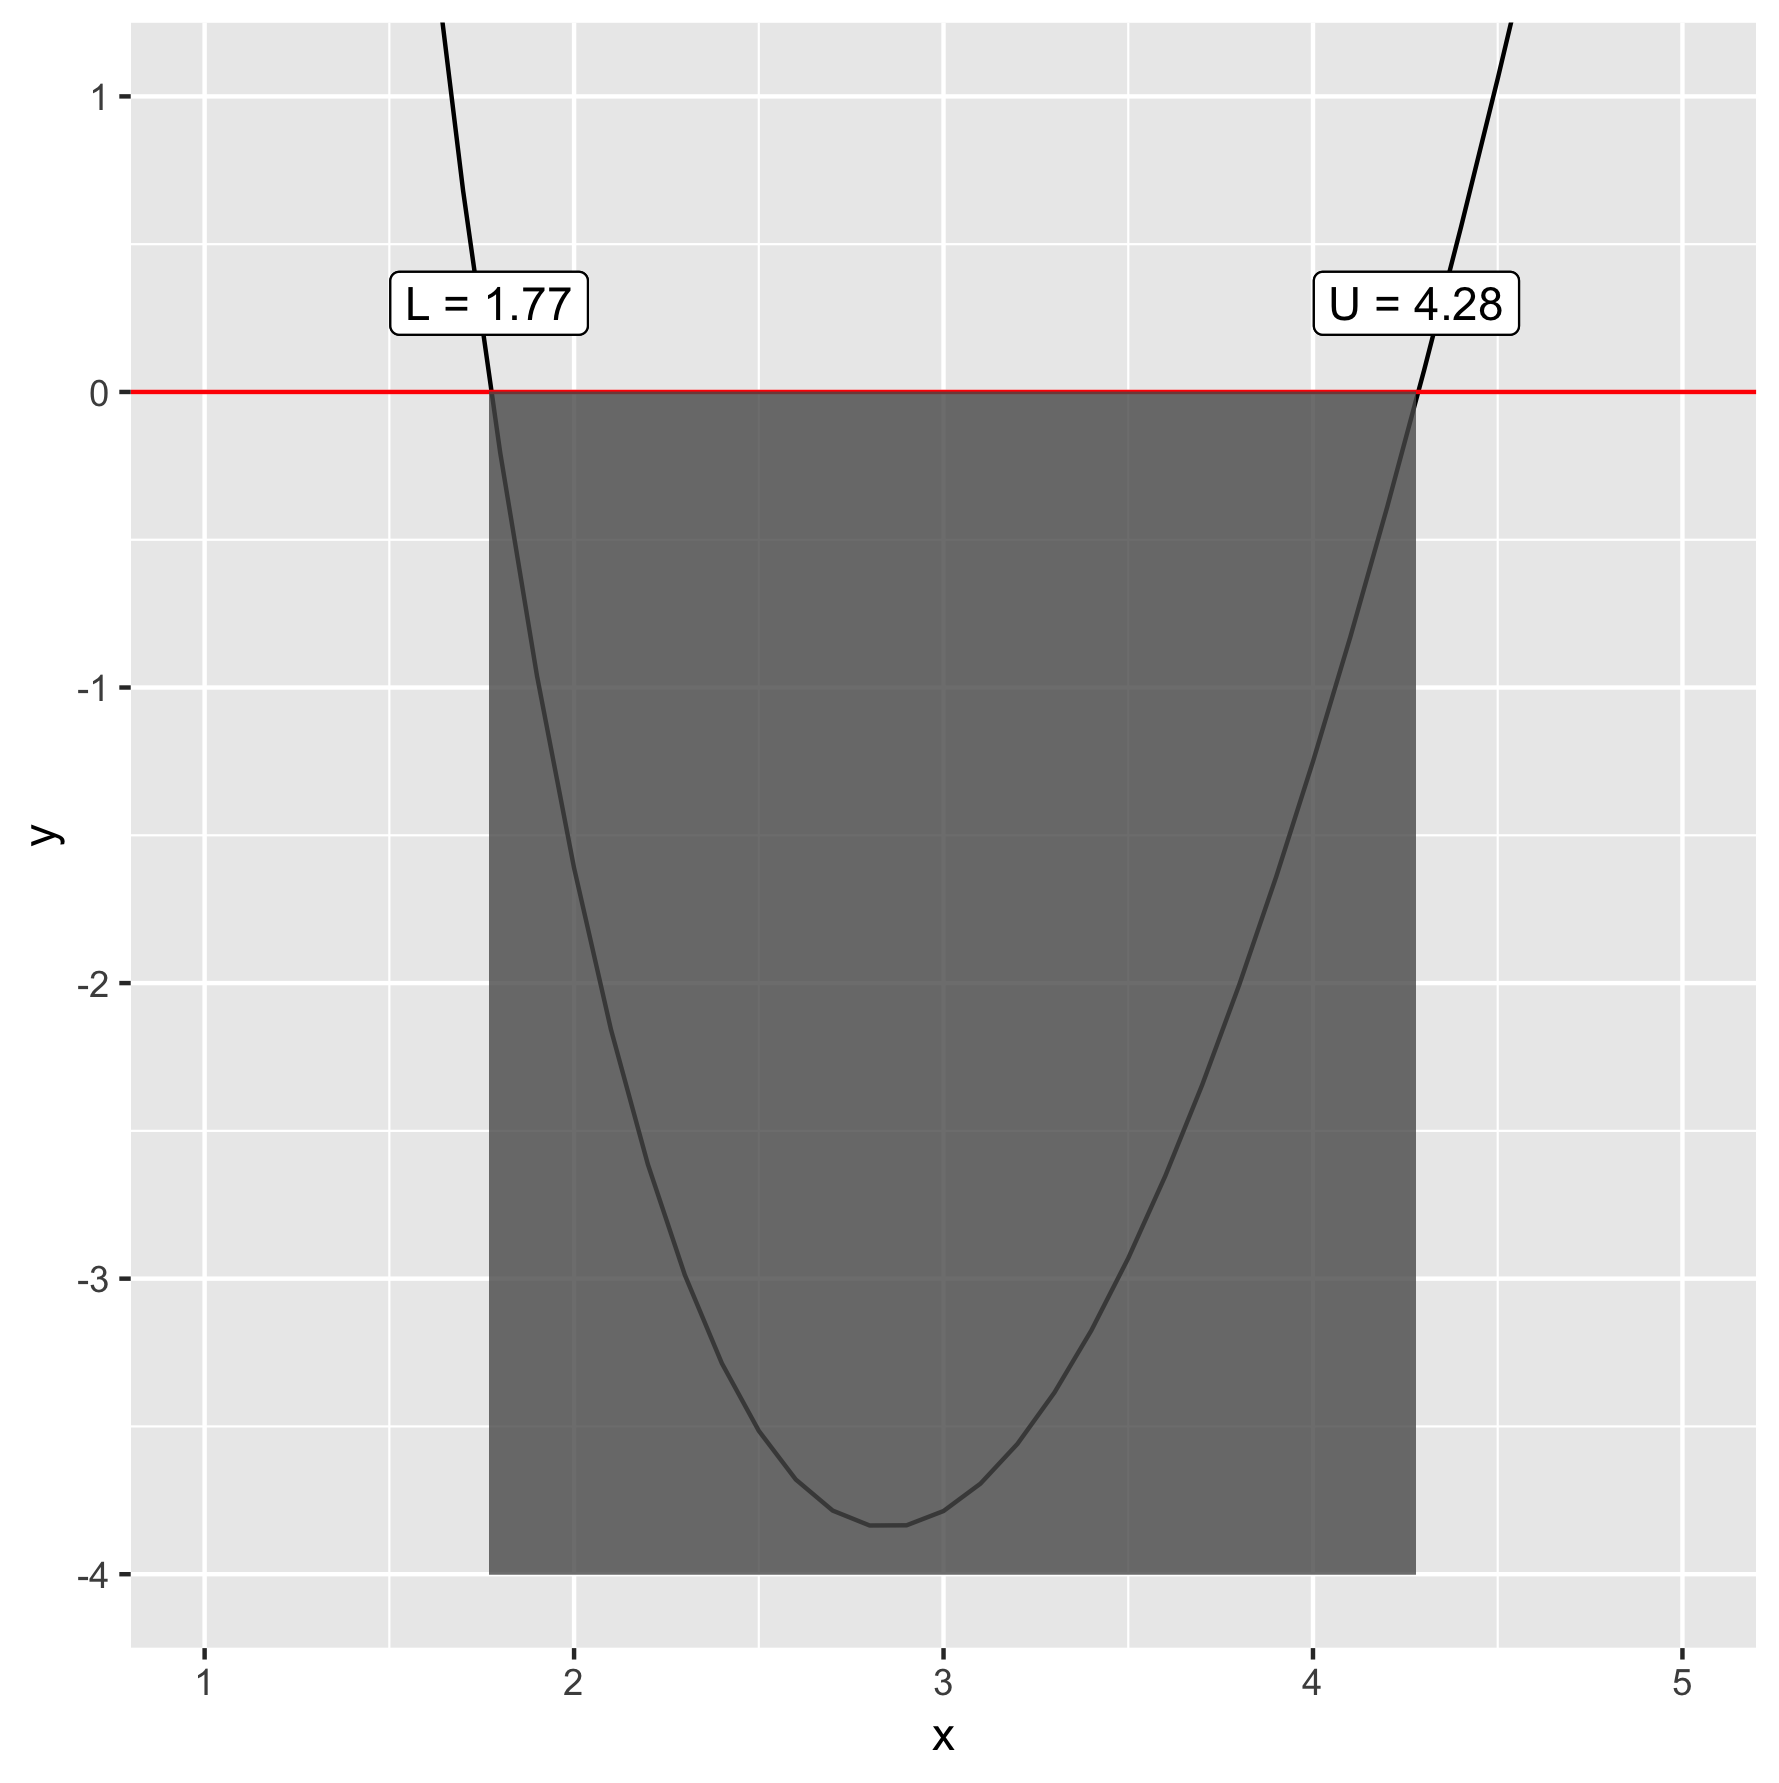
\includegraphics[scale=0.07]{src/Q13-57_visualisation.png}
\end{center}

\section{Sélection de modèles}
\subsection*{Chi-Square \emph{Goodness-of-fit}}
On veut valider l'adéquation du modèle qu'on propose avec ce test. On calcule la quantité $X^2$ : 
\[X^2 = \frac{\sum_{j=1}^{k}(E_j - O_j)^2 }{E_j}\]
où $E_j = n \hat{p}_i$ est le nombre de valeurs qu'on s'attend à avoir dans la $i$\up{e} classe et $O_j = n p_{ni}$ le nombre d'observations dans la $i$\up{e} classe. On peut prouver que
\[X^2 \sim \chi_{k-p-1}^2\] \\

On peut aussi faire le test LRT pour valider l'adéquation aussi.

\subsection*{Critères de sélection}
Pour chosir entre plusieurs modèles, on peut, entre autres, se baser sur les critères suivants : 
\begin{enumerate}
\item la plus \textbf{faible valeur} pour le test \textbf{Kolmogorov-Smirnov} ; 
\item  la plus \textbf{faible valeur} pour le test \textbf{Anderson-Darling} ;
\item  la plus \textbf{faible valeur} pour le test \textbf{Goodness-of-fit} ;
\item la plus \textbf{haute valeur} pour la \textbf{\emph{p-value} du test Goodness-of-fit} ; 
\item la plus \textbf{haute valeur} pour la \textbf{fonction de vraisemblance à son maximum}.
\end{enumerate}

\section{Estimation bayésienne}
\begin{definition}[Distribution \emph{a priori}]
Soit un paramètre $\theta$ d'une distribution quelconque. Afin de réaliser une estimation Bayésienne, on connaît \emph{a priori} la distribution que prend le paramètre $\theta$, qu'on dénote par $\pi(\theta)$. \\

Alors, notre distribution des pertes est conditionnée par rapport à la valeur que $\theta$ prend (i.e. $f_{X|\Theta}$).
\end{definition}


\begin{definition}[Distribution \emph{a posteriori}]
La distribution \emph{a posteriori} nous permet de savoir avec quelle probabilité non-nulle notre paramètre $\theta$ peut prendre une certaine valeur, sachant qu'on a observé certains $x$, qu'on dénote comme $\pi_{\Theta | X}(\theta | x)$ : 
\begin{equation}
\label{eq:dist_posteriori}
\pi_{\Theta | X}(\theta | x) = \frac{f_{\Theta, X}(\theta, x)}{f_{X}(x)} = \frac{f_{X|\Theta}(x | \theta) \pi(\theta)}{\int f_{X|\Theta}(x | \theta) \pi(\theta) d \theta} 
\end{equation}
L'idée est de remplacer les différentes distributions dans l'\autoref{eq:dist_posteriori}, et en déduire une distribution avec une paramétrisation différente\footnote{Souvent, la distribution \emph{a posteriori} aura la même distribution que celle \emph{a priori}, mais avec des paramètres différents.}.
\end{definition}

\paragraph{L'estimateur Bayésien} L'estimateur Bayésien est défini comme l'espérance du paramètre $\theta$, sachant la distribution de $X$. En d'autres mots, on veut l'espérance de la distribution \emph{a posteriori} : 
\begin{equation}
\label{eq:estimateur_bayes}
\hat{\theta}_{BAYES} = \esp{\Theta | X}
\end{equation}

 \section{Rappel de probabilité}
 \subsection*{Certaines lois à savoir}
 \begin{tabular}{|a| * {4}{C|}}
 \hline
 \rowcolor{red!30!white}\text{Loi} & \prob{X = x} \text{ ou } f_X(x) & \esp{X} & Var(X) & M_X(t) \\\hline
 Bin(n,p)	& \binom{n}{x} p^x (1-p)^{n-x} & np & np(1-p) & \left( (1-p) + p^t \right)^n \\\hline
 Pois(\lambda) & \frac{e^{-\lambda} \lambda^x}{x!} & \lambda & \lambda & e^{\lambda(t-1)} \\\hline
 Gamma(\alpha, \lambda) & \frac{\lambda^{\alpha} x^{\alpha-1} e^{-\lambda x}}{\Gamma(\alpha)} & \frac{\alpha}{\lambda} & \frac{\alpha}{\lambda^2} & \left( \frac{\lambda}{\lambda - t} \right)^\alpha \\\hline
 Normale(\mu, \sigma^2) & \frac{1}{\sqrt{2 \pi} \sigma} e^{- \frac{1}{2} \left( \frac{x-\mu}{\sigma} \right)^2} & \mu & \sigma^2 & e^{\mu t + \frac{\sigma^2 t^2}{2}} \\\hline
 \end{tabular}
 
 \subsection*{Rappels d'algèbre linéaire}
\subsubsection*{Matrice transposée} la matrice transposée est définie par $\bm{A}^\top$, telle que
\begin{align*}
\bm{A}^{\top} & = 
\begin{bmatrix}
a	& -c \\
-b	& d \\
\end{bmatrix}
\end{align*}

\subsubsection*{Déterminant d'une matrice} On peut calculer le déterminant $\det(\bm{A})$ de la matrice $\bm{A}$ tel que
\begin{align*}
\det(\bm{A})	  = 
\begin{vmatrix}
a	& b \\
c	& d \\
\end{vmatrix}
= ad - bc
\end{align*}

\subsubsection*{Inverse d'une matrice} L'équivalent de l'opération $\frac{1}{\bm{A}}$ en algèbre linéaire est de calculer la matrice inverse de $\bm{A}^{-1}$, telle que
\begin{align*}
\bm{A}^{-1}	& = \frac{1}{\det(\bm{A})}
\begin{bmatrix}
a	& -c \\
-b	& d \\
\end{bmatrix}
\end{align*}
où on multiple par la matrice adjointe de $\bm{A}$. Il faut normalement calculer les cofacteurs, mais le cas à 2 dimensions est un cas simplifié.



\end{multicols*}


%% -----------------------------
%% Fin du document
%% -----------------------------
\end{document}